\documentclass[final,hyperref={pdfpagelabels=false}]{beamer}

\usepackage[orientation=portrait,size=a0,scale=1.4]{beamerposter}
\usetheme{I6pd2}
\usepackage[english]{babel}
\usepackage{amsmath,amsthm,amssymb,latexsym}
\usepackage{booktabs}
\usepackage{caption}
\usepackage{tcolorbox}
\usepackage{xcolor}
\graphicspath{{Images/}}
\usepackage[tight,footnotesize]{subfigure}

\definecolor{Blue}{HTML}{000080}

\usecaptiontemplate{\small\structure{\insertcaptionname~\insertcaptionnumber: }\insertcaption}

\title{Bayesian Nonparametric Motor-skill Representations \\ for Efficient Learning of Robotic Clothing Assistance}
\author{Nishanth Koganti$^{1,2}$, Tomoya Tamei$^1$, Kazushi Ikeda$^1$, Tomohiro Shibata$^2$}
\institute{$^1$Nara Institute of Science and Technology, Japan~~$^2$Kyushu Institute of Technology, Japan}

\newcommand{\leftfoot}{Neural Information Processing Systems 2016}
\newcommand{\rightfoot}{Workshop on Practical Bayesian Nonparametrics}

\begin{document}

\addtobeamertemplate{block end}{}{\vspace*{0.5ex}}
\addtobeamertemplate{block alerted end}{}{\vspace*{2ex}}

\begin{frame}[t]

\begin{columns}[t]

\begin{column}{.02\linewidth}\end{column}

\begin{column}{0.47\linewidth}

\begin{block}{Introduction}

\begin{center}
\textbf{Objective}: Robotic Clothing Assistance is a challenging problem involving \emph{interaction with Human and Clothing material}. In this study, we propose a method for the realtime estimation of the Human-Cloth topological relationship using a depth sensor.
\end{center}

\begin{columns}[t]

\begin{column}{0.55\linewidth}

~\\
Tamei et. al.[1] developed clothing assistance robot to perform T-shirt clothing task:\\~\\
\begin{itemize}
\item \textbf{Reinforcement Learning} scheme used to acquire motor skills for cloth handling.\\~\\
\item \textbf{Low dimensional represetations} of state and policy used to ensure fast learning time.
\end{itemize}

\end{column}

\begin{column}{0.45\linewidth}

\begin{figure}
\centering
\includegraphics[width=0.9\textwidth]{mannequin.png}
\end{figure}

\end{column}

\end{columns}

\end{block}

\end{column}

\begin{column}{0.47\linewidth}

\begin{block}{Problem Decription}

\begin{columns}[t]

\begin{column}{0.5\linewidth}
\textbf{Topology Coordinates}[2] represents interaction between two curves using low dimensional variables:

\begin{itemize}
\item \textbf{Writhe}, $w \in \mathbb{R}$
\vspace{3mm}
\item \textbf{Center}, $\text{c} = [c_1,c_2] \in \mathbb{R}^2$
\vspace{3mm}
\item \textbf{Density}, $d \in \mathbb{R}$
\end{itemize}

\vspace{3mm}

\begin{figure}
\centering
\includegraphics[width=\linewidth]{humancloth.pdf}
\end{figure}

\end{column}

\begin{column}{0.5\linewidth}

\begin{figure}
\centering
\includegraphics[width=\textwidth]{topology.png}
\end{figure}

\vspace{3mm}

\centering \textbf{Human-Cloth relationship} low dimensionally represented using topology coordinates:

\begin{itemize}
\item T-shirt collar and Mannequin's Head
\vspace{2mm}
\item T-shirt collar and Mannequin's Body
\vspace{2mm}
\item T-shirt sleeve and Mannequin's Shoulder
\end{itemize}

\end{column}

\end{columns}

\end{block}

\end{column}

\begin{column}{.02\linewidth}\end{column}

\end{columns}

\begin{columns}[t]

\begin{column}{0.02\linewidth}\end{column}

\begin{column}{0.96\linewidth}

\begin{alertblock}{Proposed Method}

\begin{columns}[t]

\begin{column}{0.24\linewidth}

\centering \textbf{Experimental Setup}

\begin{itemize}
\item Human-Cloth relationship observed using \textbf{Kinect depth sensor}.\\~\\
\item \textbf{Color markers} used on T-shirt and Mannequin to ensure robust estimation.
\end{itemize}

\vspace{6mm}

\begin{figure}
\centering
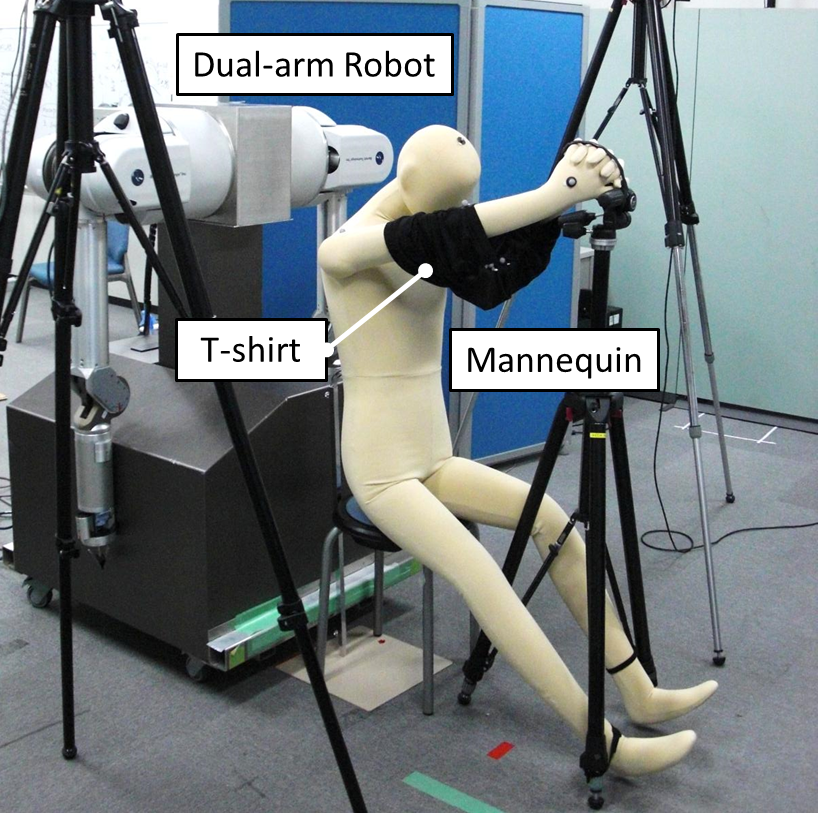
\includegraphics[width=\textwidth]{setup.png}
\end{figure}

\end{column}

\begin{column}{0.48\linewidth}

\centering \textbf{Proposed Method}

\begin{figure}
\centering
\includegraphics[width=\textwidth,height=0.22\textheight]{method.pdf}
\end{figure}

\end{column}

\begin{column}{0.24\linewidth}

\centering \textbf{T-shirt state estimation}

\vspace{3mm}

\begin{itemize}
\item T-shirt collar and sleeve shape compactly represented using \textbf{Ellipses}.\\~\\
\item Generic 3D conic fitting approach proposed Shakarji et. al.~\cite{ellipse} used for this purpose.
\end{itemize}

\vspace{3mm}

\begin{figure}
\centering
\includegraphics[width=\textwidth]{collarestimates.pdf}
\end{figure}

\end{column}

\end{columns}

\end{alertblock}

\begin{alertblock}{Experimental Results}

\begin{columns}[t]

\begin{column}{0.49\linewidth}

\centering \textbf{Robustness of Topology Space to Measurement Noise}\\
\vspace{3mm}
\centering Robustness evaluated by comparing rewards obtained in \emph{Cartesian} and \emph{Topological} space.

\begin{itemize}
\item Reward function in Cartesian Space:
\begin{equation}
r(o_t) = - \sqrt{(o_t - o_{target})^T \Sigma_o^{-1} (o_t - o_{target})}
\end{equation}
\item Reward function in Topology Space:
\begin{equation}
r(s_t) = - \sqrt{(s_t - s_{target})^T \Sigma_s^{-1} (s_t - s_{target})}
\end{equation}
\end{itemize}

\begin{columns}[t]

\begin{column}{0.49\linewidth}

\centering Simulation Experiment
\begin{figure}
\centering
\includegraphics[width=\textwidth]{toptest.pdf}
\end{figure}

\end{column}

\begin{column}{0.49\linewidth}

\begin{figure}
\centering
\includegraphics[width=\textwidth]{reward.png}
\end{figure}

\end{column}

\end{columns}

\end{column}

\begin{column}{0.49\linewidth}

\centering \textbf{Accuracy of Proposed Method}

\begin{itemize}
\item Accuracy of proposed method evaluated by comparing our estimates with the ground truth.
\vspace{3mm}
\item \textbf{Ground Truth}: Motion Capture System with 7 IR Cameras, 10 IR Markers used on T-shirt collar and 1 IR Marker on T-shirt sleeve.
\end{itemize}

\begin{columns}[t]

\begin{column}{0.59\linewidth}

\begin{figure}
\centering
\includegraphics[width=\textwidth]{realtimeresults.pdf}
\end{figure}

\end{column}

\begin{column}{0.39\linewidth}

\begin{table}
\centering
\begin{center}
\small
\begin{tabular}{ccc}
\toprule
Parameter & Pearson Corr & RMS Error\\[0.2cm]
\midrule
$s_1$ topology & 0.9364 & 0.5955\\
$s_2$ topology & 0.8857 & 0.1247\\
$s_3$ topology & 0.9889 & 0.3529\\
\bottomrule
\end{tabular}
\end{center}
\end{table}

\vspace{4mm}

\begin{itemize}
\item Proposed method provides reliable estimates in real-time (28-30 fps).
\vspace{3mm}
\item However, there are jitters due to inherent noise in depth sensor.
\end{itemize}

\end{column}

\end{columns}

\end{column}

\end{columns}

\end{alertblock}

\end{column}

\begin{column}{0.02\textwidth}\end{column}

\end{columns}

\begin{columns}[t]

\begin{column}{.02\textwidth}\end{column}

\begin{column}{0.47\textwidth}

\begin{block}{Future Work}

\begin{itemize}
\item Bayesian estimation of Human-Cloth relationship using \emph{Proprioceptive} information of robot.
\vspace{3mm}
\item Develop motor skills learning algorithm by incorporating real-time estimates.
\end{itemize}

\end{block}

\end{column}

\begin{column}{0.47\textwidth}

\begin{block}{References}

\nocite{*}
\scriptsize{
\bibliographystyle{unsrt}

\begin{thebibliography}{10}
\bibitem{tamei}
T. Tamei, T. Matsubara, A. Rai, and T. Shibata, ``Reinforcement learning of clothing assistance with a dual-arm robot'' in \emph{Proc. of the 11th IEEE-RAS Int. Conf. on Humanoid Robots, pp. 733-738,} 2011.

\bibitem{topology}
E. S. L. Ho and T. Komura, ``Character motion synthesis by topology coordinates,'' in \emph{Proc. of EUROGRAPHICS2009, vol. 28, no. 2, pp. 299-308,} 2009.

\bibitem{ellipse}
M. C. Shakarji, ``Least-squares fitting algorithms of the NIST algorithm testing system.'', in \emph{Journal of Research-National Institute of Standards and Technology 103,} 1998.
\end{thebibliography}}

\end{block}

\end{column}

\begin{column}{.02\textwidth}\end{column}

\end{columns}

\end{frame}

\end{document}
